% !TeX spellcheck = <none>
\documentclass[journal,12pt,twocolumn]{IEEEtran}
%
\usepackage{setspace}
\usepackage{gensymb}
\usepackage{caption}
%\usepackage{multirow}
%\usepackage{multicolumn}
%\usepackage{subcaption}
%\doublespacing
\usepackage{polynom}
\makeatletter
\def\pld@CF@loop#1+{%
	\ifx\relax#1\else
	\begingroup
	\pld@AccuSetX11%
	\def\pld@frac{{}{}}\let\pld@symbols\@empty\let\pld@vars\@empty
	\pld@false
	#1%
	\let\pld@temp\@empty
	\pld@AccuIfOne{}{\pld@AccuGet\pld@temp
		\edef\pld@temp{\noexpand\pld@R\pld@temp}}%
	\pld@if \pld@Extend\pld@temp{\expandafter\pld@F\pld@frac}\fi
	\expandafter\pld@CF@loop@\pld@symbols\relax\@empty
	\expandafter\pld@CF@loop@\pld@vars\relax\@empty
	\ifx\@empty\pld@temp
	\def\pld@temp{\pld@R11}%
	\fi
	\global\let\@gtempa\pld@temp
	\endgroup
	\ifx\@empty\@gtempa\else
	\pld@ExtendPoly\pld@tempoly\@gtempa
	\fi
	\expandafter\pld@CF@loop
	\fi}
\def\pld@CMAddToTempoly{%
	\pld@AccuGet\pld@temp\edef\pld@temp{\noexpand\pld@R\pld@temp}%
	\pld@CondenseMonomials\pld@false\pld@symbols
	\ifx\pld@symbols\@empty \else
	\pld@ExtendPoly\pld@temp\pld@symbols
	\fi
	\ifx\pld@temp\@empty \else
	\pld@if
	\expandafter\pld@IfSum\expandafter{\pld@temp}%
	{\expandafter\def\expandafter\pld@temp\expandafter
		{\expandafter\pld@F\expandafter{\pld@temp}{}}}%
	{}%
	\fi
	\pld@ExtendPoly\pld@tempoly\pld@temp
	\pld@Extend\pld@tempoly{\pld@monom}%
	\fi}
%
\usepackage{setspace}
\usepackage{gensymb}
\usepackage{xcolor}
\usepackage{caption}
%\usepackage{subcaption}
%\doublespacing
\singlespacing

%\usepackage{graphicx}
%\usepackage{amssymb}
%\usepackage{relsize}
\usepackage{geometry}
\usepackage[cmex10]{amsmath}
\usepackage{xfrac}
\usepackage{gensymb}
\usepackage{amssymb}
\usepackage{mathtools}
\usepackage{scalerel}
%\usepackage{amsthm}
%\interdisplaylinepenalty=2500
%\savesymbol{iint}
%\usepackage{txfonts}
%\restoresymbol{TXF}{iint}
%\usepackage{wasysym}
\usepackage{hyperref}
\usepackage{amsthm}
\usepackage{mathrsfs}
\usepackage{txfonts}
\usepackage{stfloats}
\usepackage{cite}
\usepackage{cases}
\usepackage{subfig}
%\usepackage{xtab}
\usepackage{longtable}
\usepackage{multirow}
%\usepackage{algorithm}
%\usepackage{algpseudocode}
%\usepackage{enumerate}
\usepackage{enumitem}
\usepackage{mathtools}
%\usepackage{iithtlc}
%\usepackage[framemethod=tikz]{mdframed}
\usepackage{listings}
\usepackage{polynom}


%\usepackage{stmaryrd}


%\usepackage{wasysym}
\setcounter{MaxMatrixCols}{20}
\newcommand{\longdiv}{\smash{\mkern-0.43mu\vstretch{1.31}{\hstretch{.7}{)}}\mkern-5.2mu\vstretch{1.31}{\hstretch{.7}{)}}}}
%\newcounter{MYtempeqncnt}
\DeclareMathOperator*{\Res}{Res}
%\renewcommand{\baselinestretch}{2}
\renewcommand\thesection{\arabic{section}}
\renewcommand\thesubsection{\thesection.\arabic{subsection}}
\renewcommand\thesubsubsection{\thesubsection.\arabic{subsubsection}}

\renewcommand\thesectiondis{\arabic{section}}
\renewcommand\thesubsectiondis{\thesectiondis.\arabic{subsection}}
\renewcommand\thesubsubsectiondis{\thesubsectiondis.\arabic{subsubsection}}

%\renewcommand{\labelenumi}{\textbf{\theenumi}}
%\renewcommand{\theenumi}{P.\arabic{enumi}}

% correct bad hyphenation here
\hyphenation{op-tical net-works semi-conduc-tor}

\lstset{
	language=Python,
	frame=single, 
	breaklines=true,
	columns=fullflexible
}

\begin{document}
	%
	
	\theoremstyle{definition}
	\newtheorem{theorem}{Theorem}[section]
	\newtheorem{problem}{Problem}
	\newtheorem{proposition}{Proposition}[section]
	\newtheorem{lemma}{Lemma}[section]
	\newtheorem{corollary}[theorem]{Corollary}
	\newtheorem{example}{Example}[section]
	\newtheorem{definition}{Definition}[section]
	%\newtheorem{algorithm}{Algorithm}[section]
	%\newtheorem{cor}{Corollary}
	\newcommand{\myvec}[1]{\ensuremath{\begin{pmatrix}#1\end{pmatrix}}}
	\newcommand{\BEQA}{\begin{eqnarray}}
		\newcommand{\EEQA}{\end{eqnarray}}
	\newcommand{\define}{\stackrel{\triangle}{=}}
	\bibliographystyle{IEEEtran}
	%\bibliographystyle{ieeetr}
	\providecommand{\nCr}[2]{\,^{#1}C_{#2}} % nCr
	\providecommand{\nPr}[2]{\,^{#1}P_{#2}} % nPr
	\providecommand{\mbf}{\mathbf}
	\providecommand{\pr}[1]{\ensuremath{\Pr\left(#1\right)}}
	\providecommand{\qfunc}[1]{\ensuremath{Q\left(#1\right)}}
	\providecommand{\sbrak}[1]{\ensuremath{{}\left[#1\right]}}
	\providecommand{\lsbrak}[1]{\ensuremath{{}\left[#1\right.}}
	\providecommand{\rsbrak}[1]{\ensuremath{{}\left.#1\right]}}
	\providecommand{\brak}[1]{\ensuremath{\left(#1\right)}}
	\providecommand{\lbrak}[1]{\ensuremath{\left(#1\right.}}
	\providecommand{\rbrak}[1]{\ensuremath{\left.#1\right)}}
	\providecommand{\cbrak}[1]{\ensuremath{\left\{#1\right\}}}
	\providecommand{\lcbrak}[1]{\ensuremath{\left\{#1\right.}}
	\providecommand{\rcbrak}[1]{\ensuremath{\left.#1\right\}}}
	\theoremstyle{remark}
	\newtheorem{rem}{Remark}
	\newcommand{\sgn}{\mathop{\mathrm{sgn}}}
	\providecommand{\abs}[1]{\left\vert#1\right\vert}
	\providecommand{\res}[1]{\Res\displaylimits_{#1}} 
	\providecommand{\norm}[1]{\lVert#1\rVert}
	\providecommand{\mtx}[1]{\mathbf{#1}}
	\providecommand{\mean}[1]{E\left[ #1 \right]}
	\providecommand{\fourier}{\overset{\mathcal{F}}{ \rightleftharpoons}}
	\providecommand{\ztrans}{\overset{\mathcal{Z}}{ \rightleftharpoons}}
	%\providecommand{\hilbert}{\overset{\mathcal{H}}{ \rightleftharpoons}}
	\providecommand{\system}{\overset{\mathcal{H}}{ \longleftrightarrow}}
	%\newcommand{\solution}[2]{\textbf{Solution:}{#1}}
	\newcommand{\solution}{\noindent \textbf{Solution: }}
	\providecommand{\dec}[2]{\ensuremath{\overset{#1}{\underset{#2}{\gtrless}}}}
	\numberwithin{equation}{section}
	%\numberwithin{equation}{subsection}
	%\numberwithin{problem}{subsection}
	%\numberwithin{definition}{subsection}
	\makeatletter
	\@addtoreset{figure}{problem}
	\makeatother
	\let\StandardTheFigure\thefigure
	%\renewcommand{\thefigure}{\theproblem.\arabic{figure}}
	\renewcommand{\thefigure}{\theproblem}
	%\numberwithin{figure}{subsection}
	\def\putbox#1#2#3{\makebox[0in][l]{\makebox[#1][l]{}\raisebox{\baselineskip}[0in][0in]{\raisebox{#2}[0in][0in]{#3}}}}
	\def\rightbox#1{\makebox[0in][r]{#1}}
	\def\centbox#1{\makebox[0in]{#1}}
	\def\topbox#1{\raisebox{-\baselineskip}[0in][0in]{#1}}
	\def\midbox#1{\raisebox{-0.5\baselineskip}[0in][0in]{#1}}
	\vspace{3cm}
	\title{ 
		%\logo{
			Digital Signal Processing
			%}
		%	\logo{Octave for Math Computing }
	}
	%\title{
		%	\logo{Matrix Analysis through Octave}{\begin{center}\includegraphics[scale=.24]{tlc}\end{center}}{}{HAMDSP}
		%}
	% paper title
	% can use linebreaks \\ within to get better formatting as desired
	%\title{Matrix Analysis through Octave}
	%
	%
	% author names and IEEE memberships
	% note positions of commas and nonbreaking spaces ( ~ ) LaTeX will not break
	% a structure at a ~ so this keeps an author's name from being broken across
	% two lines.
	% use \thanks{} to gain access to the first footnote area
	% a separate \thanks must be used for each paragraph as LaTeX2e's \thanks
	% was not built to handle multiple paragraphs
	%
	\author{ Omkar Raijade [EP20BTECH11020]%<-this  stops a space
		% stops a space
		%\thanks{J. Doe and J. Doe are with Anonymous University.}% <-this % stops a space
		%\thanks{Manuscript received April 19, 2005; revised January 11, 2007.}}
}
% note the % following the last \IEEEmembership and also \thanks - 
% these prevent an unwanted space from occurring between the last author name
% and the end of the author line. i.e., if you had this:
% 
% \author{....lastname \thanks{...} \thanks{...} }
%                     ^------------^------------^----Do not want these spaces!
%
% a space would be appended to the last name and could cause every name on that
% line to be shifted left slightly. This is one of those "LaTeX things". For
% instance, "\textbf{A} \textbf{B}" will typeset as "A B" not "AB". To get
% "AB" then you have to do: "\textbf{A}\textbf{B}"
% \thanks is no different in this regard, so shield the last } of each \thanks
% that ends a line with a % and do not let a space in before the next \thanks.
% Spaces after \IEEEmembership other than the last one are OK (and needed) as
% you are supposed to have spaces between the names. For what it is worth,
% this is a minor point as most people would not even notice if the said evil
% space somehow managed to creep in.
% The paper headers
%\markboth{Journal of \LaTeX\ Class Files,~Vol.~6, No.~1, January~2007}%
%{Shell \MakeLowercase{\textit{et al.}}: Bare Demo of IEEEtran.cls for Journals}
% The only time the second header will appear is for the odd numbered pages
% after the title page when using the twoside option.
% 
% *** Note that you probably will NOT want to include the author's ***
% *** name in the headers of peer review papers.                   ***
% You can use \ifCLASSOPTIONpeerreview for conditional compilation here if
% you desire.
% If you want to put a publisher's ID mark on the page you can do it like
% this:
%\IEEEpubid{0000--0000/00\$00.00~\copyright~2007 IEEE}
% Remember, if you use this you must call \IEEEpubidadjcol in the second
% column for its text to clear the IEEEpubid mark.
% make the title area
\maketitle
%\newpage
\tableofcontents
%\renewcommand{\thefigure}{\thesection.\theenumi}
%\renewcommand{\thetable}{\thesection.\theenumi}
\renewcommand{\thefigure}{\theenumi}
\renewcommand{\thetable}{\theenumi}
%\renewcommand{\theequation}{\thesection}
\bigskip
\begin{abstract}
This manual provides a simple introduction to digital signal processing.
\end{abstract}
\section{Software Installation}
Run the following commands
\begin{lstlisting}
sudo apt-get update
sudo apt-get install libffi-dev libsndfile1 python3-scipy  python3-numpy python3-matplotlib 
sudo pip install cffi pysoundfile 
\end{lstlisting}
\section{Digital Filter}
\begin{enumerate}[label=\thesection.\arabic*
,ref=\thesection.\theenumi]
\item
\label{prob:input}
Download the sound file from  
\begin{lstlisting}
	wget https://raw.githubusercontent.com/gadepall/ 
	EE1310/master/filter/codes/Sound_Noise.wav
\end{lstlisting}
%\href{http://tlc.iith.ac.in/img/sound/Sound_Noise.wav}{\url{http://tlc.iith.ac.in/img/sound/Sound_Noise.wav}}  
%in the link given below.
%\linebreak
\item
\label{prob:spectrogram}
You will find a spectrogram at \href{https://academo.org/demos/spectrum-analyzer}{\url{https://academo.org/demos/spectrum-analyzer}}. 
%\end{problem}
%%
%
%%\onecolumn
%%\input{./figs/fir}
%\begin{problem}
Upload the sound file that you downloaded in Problem \ref{prob:input} in the spectrogram  and play.  Observe the spectrogram. What do you find?
\\
%
\solution There are a lot of yellow lines between 440 Hz to 5.1 KHz.  These represent the synthesizer key tones. Also, the key strokes
are audible along with background noise.
% By observing spectrogram, it clearly shows that tonal frequency is under 4kHz. And above 4kHz only noise is present.
\item
\label{prob:output}
Write the python code for removal of out of band noise and execute the code.
\\
\solution
\lstinputlisting{/home/ubuntu/Desktop/Assign 1/noisered.py}
%\begin{figure}[h]
%\centering
%\includegraphics[width=\columnwidth]{enc_block_diag.png}
%\caption{}
%\label{fig:convolution encoder}
%\end{figure}
%\input{block_enc}
\item
The output of the python script in Problem \ref{prob:output} is the audio file Sound\_With\_ReducedNoise.wav. Play the file in the spectrogram in Problem \ref{prob:spectrogram}. What do you observe?
\\
\solution The key strokes as well as background noise is subdued in the audio.  Also,  the signal is blank for frequencies above 5.1 kHz.
\end{enumerate}
\section{Difference Equation}
\begin{enumerate}[label=\thesection.\arabic*,ref=\thesection.\theenumi]
\item Let
\label{def:xn}
\begin{equation}
	x(n) = \cbrak{\underset{\uparrow}{1},2,3,4,2,1}
\end{equation}
Sketch $x(n)$.
\item Let
\begin{multline}
	\label{eq:iir_filter}
	y(n) + \frac{1}{2}y(n-1) = x(n) + x(n-2), 
	\\
	y(n) = 0, n < 0
\end{multline}
Sketch $y(n)$.  
\\
\solution The following code yields Fig. \ref{fig:xnyn}.
\begin{lstlisting}
	wget https://github.com/gadepall/EE1310/raw/master/filter/codes/xnyn.py
\end{lstlisting}
\begin{figure}[!ht]
	\begin{center}
		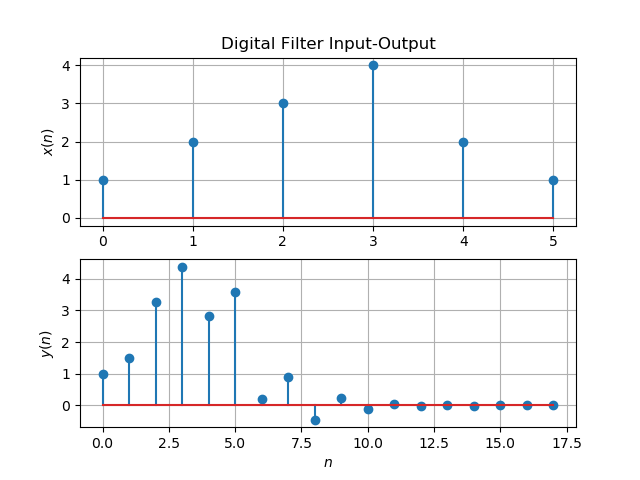
\includegraphics[width=\columnwidth]{/home/ubuntu/Desktop/Assign 1/sketchfn.png}
	\end{center}
	\captionof{figure}{}
	\label{fig:xnyn}	
\end{figure}
\item Repeat the above exercise using a C code.
\end{enumerate}
\solution
C code for creating .dat files:
\lstinputlisting{/home/ubuntu/Desktop/Assign 1/sketchfn.c}
Python code for plotting from the .dat files:
\lstinputlisting{/home/ubuntu/Desktop/Assign 1/sketchfn.py}
\section{$Z$-transform}
\begin{enumerate}[label=\thesection.\arabic*]
\item The $Z$-transform of $x(n)$ is defined as
%
\begin{equation}
	\label{eq:z_trans}
	X(z)={\mathcal {Z}}\{x(n)\}=\sum _{n=-\infty }^{\infty }x(n)z^{-n}
\end{equation}
%
Show that
\begin{equation}
	\label{eq:shift1}
	{\mathcal {Z}}\{x(n-1)\} = z^{-1}X(z)
\end{equation}
and find
\begin{equation}
	{\mathcal {Z}}\{x(n-k)\} 
\end{equation}
\solution From \eqref{eq:z_trans},
\begin{align}
	{\mathcal {Z}}\{x(n-1)\} &=\sum _{n=-\infty }^{\infty }x(n-1)z^{-n}
	\\
	&=\sum _{n=-\infty }^{\infty }x(n)z^{-n-1} = z^{-1}\sum _{n=-\infty }^{\infty }x(n)z^{-n}
\end{align}
resulting in \eqref{eq:shift1}. Similarly, it can be shown that
%
\begin{equation}
	\label{eq:z_trans_shift}
	{\mathcal {Z}}\{x(n-k)\} = z^{-k}X(z)
\end{equation}
\begin{equation}
	\text{let } y(n) = x(n-k)
\end{equation}
\begin{equation}
	Y(z) = {\mathcal {Z}}\{y(n)\} = \sum_{n=-\infty}^{\infty}y(n)z^{-n}
\end{equation}
\begin{equation}
	\implies Y(z) = \sum_{n=-\infty}^{\infty}x(n-k)z^{-n}
\end{equation}
\begin{equation}
	\text{put }n-k = p
\end{equation}
\begin{equation}
	Y(z) = \sum_{p=-\infty}^{\infty}x(p)z^{-(p+k)}
\end{equation}
\begin{equation}
	Y(z) = {\mathcal {Z}}\{y(n)\} = z^{-k}\sum_{p=-\infty}^{\infty}x(p)z^{-p}
\end{equation}
\begin{equation}
	{\mathcal{Z}}\{x(n-k)\} = z^{-k}\sum_{n=-\infty}^{\infty}x(n)z^{-n}
\end{equation}
\begin{equation}
	\boxed{{\mathcal{Z}}\{x(n-k)\} = z^{-k}X(z)}
\end{equation}
\item Obtain $X(z)$ for $x(n)$ defined in problem 
\ref{def:xn}.
\solution
\begin{equation}
	X(z) = {\mathcal{Z}}\{x(n)\} = \sum_{n=-\infty}^{\infty}x(n)z^{-n}
\end{equation}
\text{From }\eqref{def:xn}
\begin{equation}
	X(z) = \sum_{n=0}^{5}x(n)z^{-n}
\end{equation}
\begin{align}
	X(z) = x(0)z^{0} + x(1)z^{-1} + x(2)z^{-2} +\\x(3)z^{-3} + x(4)z^{-4} + x(5)z^{-5}
\end{align}
\begin{equation}
	\boxed{X(z) = 1 + 2z^{-1} + 3z^{-2} + 4z^{-3} + 2z^{-4} + z^{-5}}
\end{equation}
\item Find
%
\begin{equation}
	H(z) = \frac{Y(z)}{X(z)}
\end{equation}
%
from  \eqref{eq:iir_filter} assuming that the $Z$-transform is a linear operation.
\\
\solution  Applying \eqref{eq:z_trans_shift} in \eqref{eq:iir_filter},
\begin{align}
	Y(z) + \frac{1}{2}z^{-1}Y(z) &= X(z)+z^{-2}X(z)
	\\
	\implies H(z) = \frac{Y(z)}{X(z)} &= \frac{1 + z^{-2}}{1 + \frac{1}{2}z^{-1}}
	\label{eq:freq_resp}
\end{align}
%
\item Find the Z transform of 
\begin{equation}
	\delta(n)
	=
	\begin{cases}
		1 & n = 0
		\\
		0 & \text{otherwise}
	\end{cases}
\end{equation}
and show that the $Z$-transform of
\begin{equation}
	\label{eq:unit_step}
	u(n)
	=
	\begin{cases}
		1 & n \ge 0
		\\
		0 & \text{otherwise}
	\end{cases}
\end{equation}
is
\begin{equation}
	U(z) = \frac{1}{1-z^{-1}}, \quad \abs{z} > 1
\end{equation}
\solution It is easy to show that
\begin{equation}
	\delta(n) \ztrans 1
\end{equation}
and from \eqref{eq:unit_step},
\begin{align}
	U(z) &= \sum _{n= 0}^{\infty}z^{-n}
	\\
	&=\frac{1}{1-z^{-1}}, \quad \abs{z} > 1
\end{align}
using the fomula for the sum of an infinite geometric progression.
%
\item Show that 
\begin{equation}
	\label{eq:anun}
	a^nu(n) \ztrans \frac{1}{1-az^{-1}} \quad \abs{z} > \abs{a}
\end{equation}
\solution
\begin{equation}
	\label{eq:unit_step}
	a^{n}u(n)
	=
	\begin{cases}
		a^{n} & n \ge 0
		\\
		0 & \text{otherwise}
	\end{cases}
\end{equation}
\begin{equation}
	{\mathcal{Z}}\{a^{n}u(n)\} = \sum_{n=0}^{\infty}a^{n}z^{-n}
\end{equation}
\begin{equation}
	a^{n}u(n) \ztrans \frac{1}{1-az^{-1}} \quad \abs{z} > \abs{a}
\end{equation}
%
\item 
Let
\begin{equation}
	H\brak{e^{\j \omega}} = H\brak{z = e^{\j \omega}}.
\end{equation}
Plot $\abs{H\brak{e^{\j \omega}}}$.  Is it periodic? If so, find the period. $H(e^{\j \omega})$ is
known as the {\em Discret Time Fourier Transform} (DTFT) of $h(n)$.
\\
\solution The following code plots Fig. \ref{fig:dtft}.
\begin{lstlisting}
	wget https://raw.githubusercontent.com/gadepall/EE1310/master/filter/codes/dtft.py
\end{lstlisting}
\begin{figure}[!ht]
	\centering
	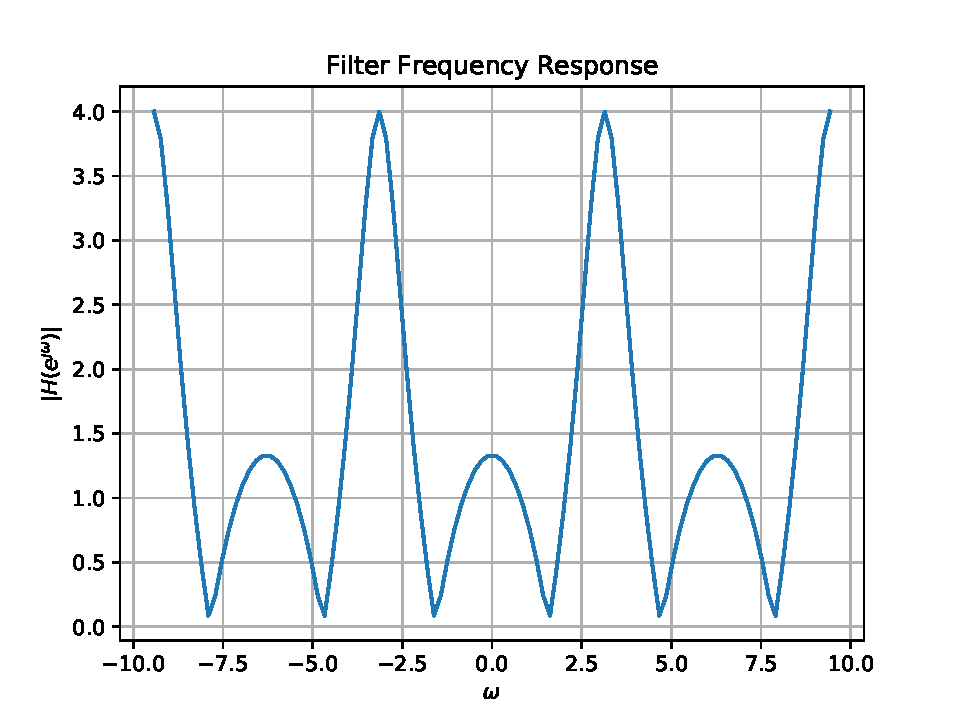
\includegraphics[width=\columnwidth]{/home/ubuntu/Desktop/Assign 1/dtft.pdf}
	\caption{$\abs{H\brak{e^{\j\omega}}}$}
	\label{fig:dtft}
\end{figure}
\solution
\begin{equation}
	H(e^{\j\omega}) = \frac{1 + e^{-2\j\omega}}{1 + \frac{1}{2}e^{-\j\omega}}
\end{equation}
\begin{equation}
	H(e^{\j\omega}) = \frac{1 + \cos2\omega - \i\sin2\omega}{1 + \frac{1}{2}\brak{\cos\omega - \i\sin\omega}}
\end{equation}
1. $\brak{1 + \cos2\omega - \i\sin2\omega}$ is periodic with period $\pi$ \\
2. $\brak{1 + \frac{1}{2}\brak{\cos\omega - \i\sin\omega}}$ is periodic with period 2$\pi$ \\
Hence, $H(e^{\j\omega})$ is periodic with period LCM($\pi$,2$\pi$) which is 2$\pi$
\item Express $h(n)$ in terms of $H\brak{e^{\j \omega}}$.
\end{enumerate}
\solution
Proof of inverse dtft:
\begin{equation}
		H(e^{\j\omega}) = \sum_{n=-\infty}^{\infty}h(n)e^{-\j\omega{n}}
\end{equation}
Multiplying both sides with $e^{\j\omega{k}}$ and integrating from $-\pi$ to $\pi$ with respect to $\omega$ we get:
\begin{equation}
	\int_{-\pi}^{\pi}H(e^{\j\omega})e^{\j\omega{k}}d\omega = \sum_{n=-\infty}^{\infty}h(n)\int_{-\pi}^{\pi}e^{-\j\omega{n}}e^{\j\omega{k}}d\omega
\end{equation}
Case 1: $n = k$
\begin{equation}
	\int_{-\pi}^{\pi}H(e^{\j\omega})e^{\j\omega{k}}d\omega = h(k)\int_{-\pi}^{\pi}d\omega
\end{equation}
\begin{equation}
	\int_{-\pi}^{\pi}H(e^{\j\omega})e^{\j\omega{k}}d\omega = 2\pi{h(k)}
\end{equation}
\begin{equation}
	\implies h(k) = \frac{1}{2\pi}\int_{-\pi}^{\pi}H(e^{\j\omega})e^{\j\omega{k}}d\omega
\end{equation}
Case 2: $n \neq k$
\begin{equation}
	\int_{-\pi}^{\pi}H(e^{\j\omega})e^{\j\omega{k}}d\omega = \sum_{n=-\infty}^{\infty}h(n)\int_{-\pi}^{\pi}e^{\j\omega{(k-n)}}d\omega
\end{equation}
\begin{align}
	= \sum_{n=-\infty}^{\infty}h(n)\frac{e^{\j\omega{(k-n)}}}{\j{(k-n)}} \quad \text{from $-\pi$ to $\pi$}
\end{align}
\begin{align}
	= \sum_{n=-\infty}^{\infty}\frac{h(n)}{\j{(k-n)}}\left[e^{\j\pi{(k-n)}} - e^{-\j\pi{(k-n)}}\right]
\end{align}
\begin{align}
	= \sum_{n=-\infty}^{\infty}\frac{h(n)}{\j{(k-n)}}\left[\cos\pi{(k-n)} - \cos\pi{(k-n)}\right]
\end{align}
\begin{align}
	\int_{-\pi}^{\pi}H(e^{\j\omega})e^{\j\omega{k}}d\omega = 0
\end{align}
\begin{equation}
	\boxed{h(n) = \frac{1}{2\pi}\int_{-\pi}^{\pi}H(e^{\j\omega})e^{\j\omega{n}}d\omega}
\end{equation}
\\Solving for $h(n)$:
\begin{equation}
	H(e^{\j\omega}) = \frac{1 + e^{-\j2\omega}}{1 + \frac{1}{2}e^{-\j\omega}}
\end{equation}
\begin{equation}
	H(z) = \frac{1 + z^{-2}}{1 + \frac{1}{2}z^{-1}}
\end{equation}
\begin{equation}
	H(z) = (1 + z^{-2})\brak{1 + \frac{1}{2}z^{-1}}^{-1}
\end{equation}
\begin{equation}
	H(z) = \brak{1 + z^{-2}}\brak{1 + \frac{1}{2z}}^{-1}
\end{equation}
\begin{equation}
	H(z) = \brak{1 + z^{-2}}\brak{1 - \frac{1}{2z} + \frac{1}{(2z)^{2}} - \frac{1}{(2z)^{3}} + ...}
\end{equation}
\begin{equation}
	H(z) = \brak{1 + z^{-2}}\brak{1 - \frac{z^{-1}}{2} + \frac{z^{-2}}{4} - \frac{z^{-3}}{8} + ...}
\end{equation}
\begin{align*}
	H(z) = \brak{1 - \frac{z^{-1}}{2} + \frac{z^{-2}}{4} - \frac{z^{-3}}{8} + ...} \\+ \brak{z^{-2} - \frac{z^{-3}}{2} + \frac{z^{-4}}{4} - ...}
\end{align*}
\begin{equation}
	H(z) = 1 - \frac{z^{-1}}{2} + \frac{5}{4}z^{-2} - \frac{5}{8}z^{-3} + \frac{5}{16}z^{-4} - ...
\end{equation}
\begin{equation}
	H(e^{\j\omega}) = 1 - \frac{e^{-\j\omega}}{2} + \frac{5}{4}e^{-\j2\omega} - \frac{5}{8}e^{-\j3\omega} + \frac{5}{16}e^{-\j4\omega} - ...
\end{equation}
\text{We have proved earlier that: }
\begin{equation}
	h(n) = \frac{1}{2\pi}\int_{-\pi}^{\pi}H(e^{\j\omega})e^{\j\omega{n}}d\omega
\end{equation}
\text{Therefore}
\begin{equation}
	\boxed{h(n) = \bigg\{1, \frac{-1}{2}, \frac{5}{4}, \frac{-5}{8}, \frac{5}{16}, \frac{-5}{32}, ...\bigg\}}
\end{equation}
\section{Impulse Response}
\begin{enumerate}[label=\thesection.\arabic*]
\item Using long division, 
find
\begin{align}
	h(n), \quad n < 5
\end{align}
for H(z) in 
\eqref{eq:freq_resp}. \\
\solution
\begin{equation}
	H(z) = \frac{1 + z^{-2}}{1 + \frac{1}{2}z^{-1}}
\end{equation}
The ROC is $|z| > \frac{1}{2}$
\[
\arraycolsep=1pt
\renewcommand\arraystretch{1.2}
\begin{array}{*1r @{\hskip\arraycolsep}c@{\hskip\arraycolsep} *{11}r}
	&          & 1 & - & \frac{1}{2}z^{-1}   \\
	\cline{2-13}
	1+\frac{1}{2}z^{-1} & \longdiv & 1 & + & z^{-2} &   &      &   &      &   &      &   &        \\
	&          & 1 & + & \frac{1}{2}z^{-1} &   &      &   &      &   &        \\
	\cline{3-7}
	&          &   &   & -\frac{1}{2}z^{-1} & + &  z^{-2} &   &      &   &      &   &        \\
	&          &   &   & -\frac{1}{2}z^{-1} & - & \frac{1}{4}z^{-2} &  &   &      &   &        \\
	\cline{5-9}
	&          &   &   &   &   & \frac{5}{4}z^{-2} &   &      &   &        \\
\end{array}
\]
\begin{equation}
	H(z) = \brak{1 - \frac{1}{2}z^{-1}} + \frac{\frac{5}{4}z^{-2}}{\brak{1 + \frac{1}{2}z^{-1}}}
\end{equation}
\begin{equation}
	= \brak{1 - \frac{1}{2}z^{-1}} + \frac{5}{4}z^{-2}{\brak{1 + \frac{1}{2}z^{-1}}}^{-1}
\end{equation}
\begin{align*}
	= \brak{1 - \frac{1}{2}z^{-1}} +\\ \frac{5}{4}z^{-2}\brak{1 - \frac{z^{-1}}{2} + \frac{z^{-2}}{4} - \frac{z^{-3}}{8} ...}
\end{align*}
\begin{align}
	= 1 - \frac{1}{2}z^{-1} + \frac{5}{4}z^{-2} - \frac{5}{8}z^{-3} + \frac{5}{16}z^{-4}
\end{align}
For $n < 5$
\begin{equation}
	h(n) = \left\{1, -\frac{1}{2}, \frac{5}{4}, -\frac{5}{8}, \frac{5}{16}\right\}
\end{equation}
\item \label{prob:impulse_resp}
Find an expression for $h(n)$ using $H(z)$, given that 
%in Problem \ref{eq:ztransab} and \eqref{eq:anun}, given that
\begin{equation}
	\label{eq:impulse_resp}
	h(n) \ztrans H(z)
\end{equation}
and there is a one to one relationship between $h(n)$ and $H(z)$. $h(n)$ is known as the {\em impulse response} of the
system defined by \eqref{eq:iir_filter}.
\\
\solution From \eqref{eq:freq_resp},
\begin{align}
	H(z) &= \frac{1}{1 + \frac{1}{2}z^{-1}} + \frac{ z^{-2}}{1 + \frac{1}{2}z^{-1}}
	\\
	\implies h(n) &= \brak{-\frac{1}{2}}^{n}u(n) + \brak{-\frac{1}{2}}^{n-2}u(n-2)
\end{align}
using \eqref{eq:anun} and \eqref{eq:z_trans_shift}.
\item Sketch $h(n)$. Is it bounded? Justify theoretically.
\\
\solution The following code plots Fig. \ref{fig:hn}.
\begin{lstlisting}
	wget https://raw.githubusercontent.com/gadepall/EE1310/master/filter/codes/hn.py
\end{lstlisting}
\begin{figure}[!ht]
	\centering
	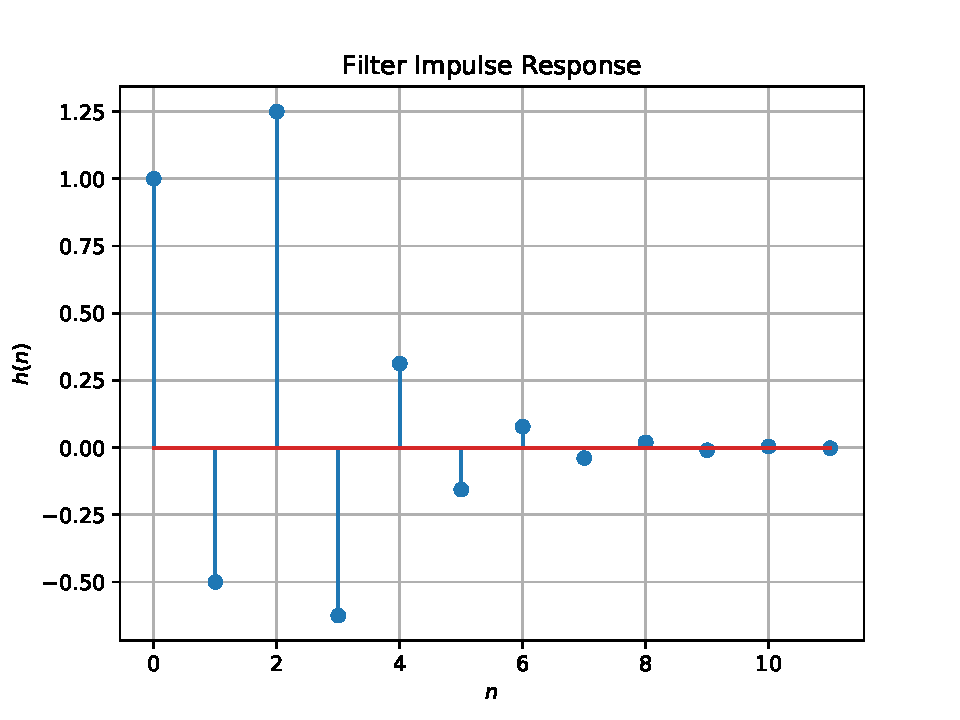
\includegraphics[width=\columnwidth]{/home/ubuntu/Desktop/Assign 1/hn.pdf}
	\caption{$h(n)$ as the inverse of $H(z)$}
	\label{fig:hn}
\end{figure}
Yes, it is bounded. The supremum is $\frac{5}{4}$ and the infrimum is $-\frac{5}{8}$ as all other points of the sequence lie in between these two which can be easily observed. \\
\item Convergent? Justify using the ratio test. \\
\solution 
$h(n)$ is:
\begin{equation}
	h(n) = \brak{-\frac{1}{2}}^{n}u(n) + \brak{-\frac{1}{2}}^{n-2}u(n-2)
\end{equation}
Ratio test:
\begin{equation}
	L = \lim_{n \to \infty}\abs{\frac{h(n+1)}{h(n)}} = \abs{\frac{\brak{-\frac{1}{2}}^{n+1} + \brak{-\frac{1}{2}}^{n-1}}{\brak{-\frac{1}{2}}^{n} + \brak{-\frac{1}{2}}^{n-2}}}
\end{equation}
\begin{equation}
	L = \abs{\frac{-\frac{1}{2}\left[{\brak{-\frac{1}{2}}^{n} + \brak{-\frac{1}{2}}^{n-2}}\right]}{{\brak{-\frac{1}{2}}^{n} + \brak{-\frac{1}{2}}^{n-2}}}}
\end{equation}
\begin{equation}
	L = \abs{-\frac{1}{2}}
\end{equation}
\begin{equation}
	L = \frac{1}{2}
\end{equation}
As $L < 1$, the series is convergent. \\
\item The system with $h(n)$ is defined to be stable if
\begin{equation}
	\sum_{n=-\infty}^{\infty}h(n) < \infty
\end{equation}
Is the system defined by \eqref{eq:iir_filter} stable for the impulse response in \eqref{eq:impulse_resp}? \\
\solution
$h(n)$ is zero for $n<0$, hence:
\begin{equation}
	\sum_{n=-\infty}^{\infty}h(n) = \sum_{n=0}^{\infty}h(n)
\end{equation}
\begin{equation}
	= 1 - \frac{1}{2} + \frac{5}{4} - \frac{5}{8} + \frac{5}{16} - \frac{5}{32} + ...
\end{equation}
\begin{equation}
	= \frac{1}{2} + \frac{5}{4}\left(1 - \frac{1}{2} + \frac{1}{4} - \frac{1}{8} + ...\right)
\end{equation}
\begin{equation}
	= \frac{1}{2} + \frac{5}{4}\left(\frac{1}{1 + \frac{1}{2}}\right)
\end{equation}
\begin{equation}
	= \frac{4}{3}
\end{equation}
\begin{equation}
	\implies \sum_{n=-\infty}^{\infty}h(n) = \frac{4}{3} < \infty
\end{equation}
Hence the system is stable. \\
%
\item Verify the above result using a python code. \\
\solution
The following Python code verifies above result:
\begin{lstlisting}
	wget https://github.com/omkar30122001/Assign_1/blob/main/sumhn.py
\end{lstlisting}
\item 
Compute and sketch $h(n)$ using 
\begin{equation}
	\label{eq:iir_filter_h}
	h(n) + \frac{1}{2}h(n-1) = \delta(n) + \delta(n-2), 
\end{equation}
%
This is the definition of $h(n)$.
\\
\solution The following code plots Fig. \ref{fig:hndef}. Note that this is the same as Fig. 
\ref{fig:hn}. 
%
\begin{lstlisting}
	wget https://raw.githubusercontent.com/gadepall/EE1310/master/filter/codes/hndef.py
\end{lstlisting}
\begin{figure}[!ht]
	\centering
	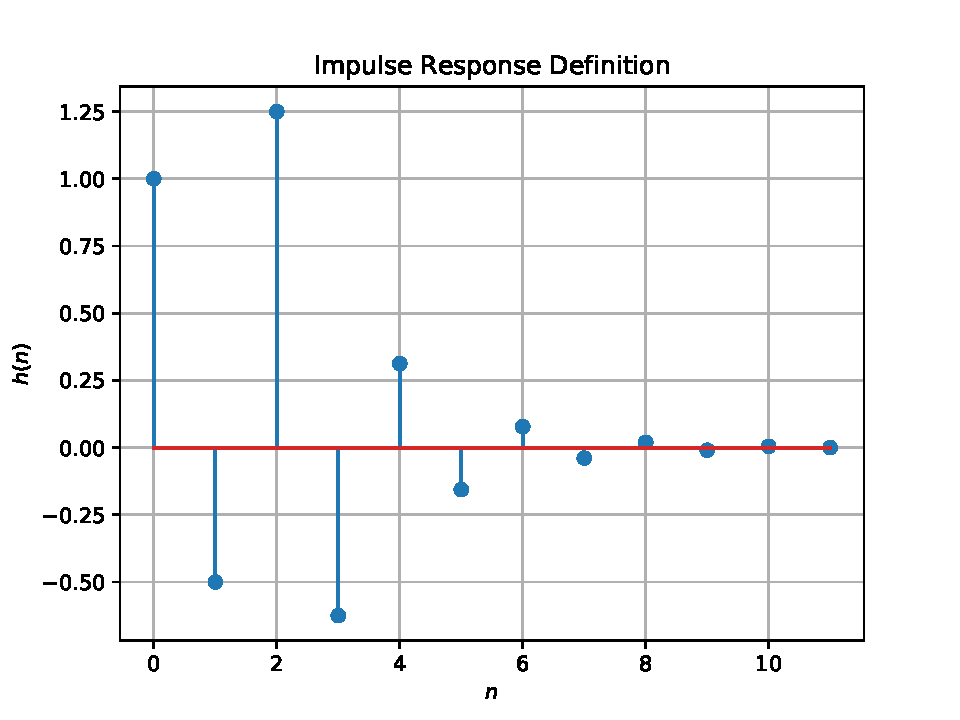
\includegraphics[width=\columnwidth]{/home/ubuntu/Desktop/Assign 1/hndef.pdf}
	\caption{$h(n)$ from the definition}
	\label{fig:hndef}
\end{figure}
%
\item Compute 
%
\begin{equation}
	\label{eq:convolution}
	y(n) = x(n)*h(n) = \sum_{n=-\infty}^{\infty}x(k)h(n-k)
\end{equation}
%
Comment. The operation in \eqref{eq:convolution} is known as
{\em convolution}.
%
\\
\solution The following code plots Fig. \ref{fig:ynconv}. Note that this is the same as 
$y(n)$ in  Fig. 
\ref{fig:xnyn}. 
%
\begin{lstlisting}
	wget https://raw.githubusercontent.com/gadepall/EE1310/master/filter/codes/ynconv.py
\end{lstlisting}
\begin{figure}[!ht]
	\centering
	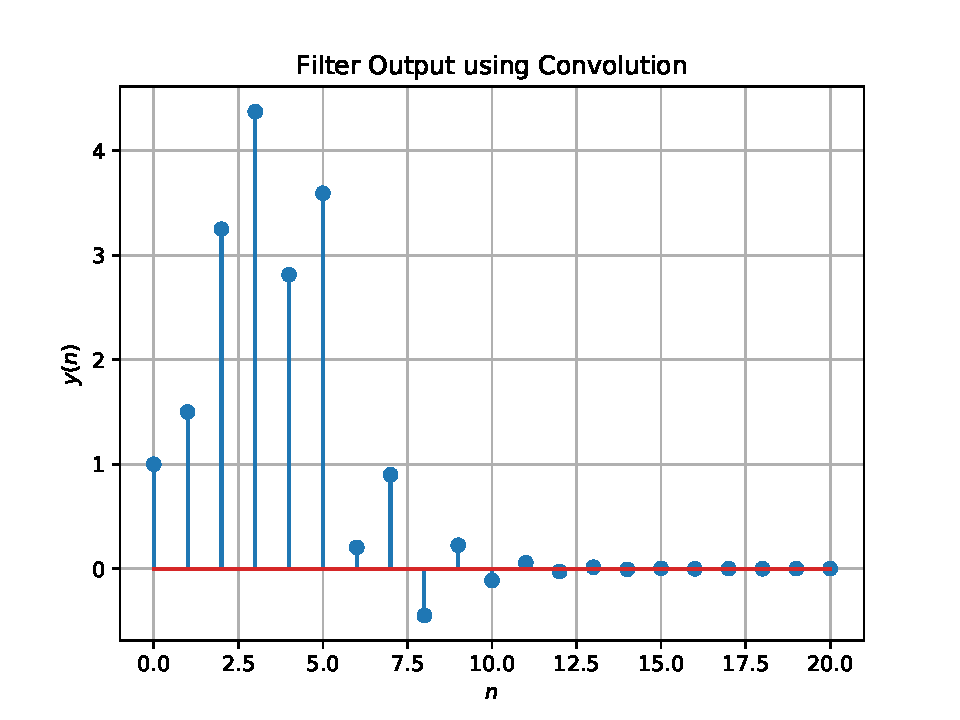
\includegraphics[width=\columnwidth]{/home/ubuntu/Desktop/Assign 1/ynconv.pdf}
	\caption{$y(n)$ from the definition of convolution}
	\label{fig:ynconv}
\end{figure}
\item Express the above convolution using a Teoplitz matrix. \\
\solution \\
\begin{equation}
	y(n) = 
	\left(
	\begin{smallmatrix}
		h(0) & 0 & 0 & 0 & 0 & 0 \\
		h(1) & h(0) & 0 & 0 & 0 & 0 \\
		h(2) & h(1) & h(0) & 0 & 0 & 0 \\
		h(3) & h(2) & h(1) & h(0) & 0 & 0 \\
		h(4) & h(3) & h(2) & h(1) & h(0) & 0 \\
		h(5) & h(4) & h(3) & h(2) & h(1) & h(0) \\
		h(6) & h(5) & h(4) & h(3) & h(2) & h(1) \\
		h(7) & h(6) & h(5) & h(4) & h(3) & h(2) \\
		h(8) & h(7) & h(6) & h(5) & h(4) & h(3) \\
		h(9) & h(8) & h(7) & h(6) & h(5) & h(4) \\
		h(10) & h(9) & h(8) & h(7) & h(6) & h(5) \\
		\vdots & \vdots & \vdots & \vdots & \vdots & \vdots \\
	\end{smallmatrix}
	\right)
	\left(
	\begin{smallmatrix}
		1 \\ 2 \\ 3 \\ 4 \\ 2 \\ 1 \\
	\end{smallmatrix}
	\right)
\end{equation}
\begin{equation}
	y(n) = 
	\left(
	\begin{smallmatrix}
		1 & 0 & 0 & 0 & 0 & 0 \\
		\sfrac{-1}{2} & 1 & 0 & 0 & 0 & 0 \\
		\sfrac{5}{4} & \sfrac{-1}{2} & 1 & 0 & 0 & 0 \\
		\sfrac{-5}{8} & \sfrac{5}{4} & \sfrac{-1}{2} & 1 & 0 & 0 \\
		\sfrac{5}{16} & \sfrac{-5}{8} & \sfrac{5}{4} & \sfrac{-1}{2} & 1 & 0 \\
		\sfrac{-5}{32} & \sfrac{5}{16} & \sfrac{-5}{8} & \sfrac{5}{4} & \sfrac{-1}{2} & 1 \\
		\sfrac{5}{64} & \sfrac{-5}{32} & \sfrac{5}{16} & \sfrac{-5}{8} & \sfrac{5}{4} & \sfrac{-1}{2} \\
		\sfrac{-5}{128} & \sfrac{5}{64} & \sfrac{-5}{32} & \sfrac{5}{16} & \sfrac{-5}{8} & \sfrac{5}{4} \\
		\sfrac{5}{256} & \sfrac{-5}{128} & \sfrac{5}{64} & \sfrac{-5}{32} & \sfrac{5}{16} & \sfrac{-5}{8} \\
		\sfrac{-5}{512} & \sfrac{5}{256} & \sfrac{-5}{128} & \sfrac{5}{64} & \sfrac{-5}{32} & \sfrac{5}{16} \\
		\sfrac{5}{1024} & \sfrac{-5}{512} & \sfrac{5}{256} & \sfrac{-5}{128} & \sfrac{5}{64} & \sfrac{-5}{32} \\
		\vdots & \vdots & \vdots & \vdots & \vdots & \vdots \\
	\end{smallmatrix}
	\right)
	\left(
	\begin{smallmatrix}
		1 \\ 2 \\ 3 \\ 4 \\ 2 \\ 1 \\
	\end{smallmatrix}
	\right)
\end{equation}
\begin{equation}
	y(n) = 
	\left(
	\begin{smallmatrix}
		1 \\ \sfrac{3}{2} \\ \sfrac{13}{4} \\ \sfrac{35}{8} \\ \sfrac{35}{16} \\ \sfrac{115}{32} \\ \sfrac{13}{64} \\ \sfrac{115}{128} \\ \sfrac{-115}{256} \\ \sfrac{115}{512} \\ \sfrac{-115}{1024} \\
	\end{smallmatrix}
	\right)
\end{equation}
\item Show that
\begin{equation}
	y(n) =  \sum_{n=-\infty}^{\infty}x(n-k)h(k)
\end{equation}
\solution
From \eqref{eq:convolution} we have
\begin{equation}
	y(n) = \sum_{n=-\infty}^{\infty}x(k)h(n-k)
\end{equation}
Replace $n$ by $m+k$
\begin{equation}
	y(m+k) = \sum_{m+k=-\infty}^{\infty}x(k)h(m)
\end{equation}
Now replace $k$ by $n-m$
\begin{equation}
	y(n) = \sum_{n=-\infty}^{\infty}x(n-m)h(m)
\end{equation}
\begin{equation}
	\implies \boxed{y(n) = \sum_{n=-\infty}^{\infty}x(n-k)h(k)}
\end{equation}
\end{enumerate}
%
\section{DFT}

\begin{enumerate}[label=\thesection.\arabic*
	,ref=\thesection.\theenumi]
	\item
Compute
\begin{equation}
	X(k) \define \sum _{n=0}^{N-1}x(n) e^{-\j2\pi kn/N}, \quad k = 0,1,\dots, N-1
\end{equation}
and $H(k)$ using $h(n)$.\\
\solution The following code plots Fig. \ref{fig:6.1}.
	%
\begin{lstlisting}
wget https://github.com/omkar30122001/Assign_1/blob/main/6.1.py
\end{lstlisting}
\begin{figure}[!ht]
	\centering
	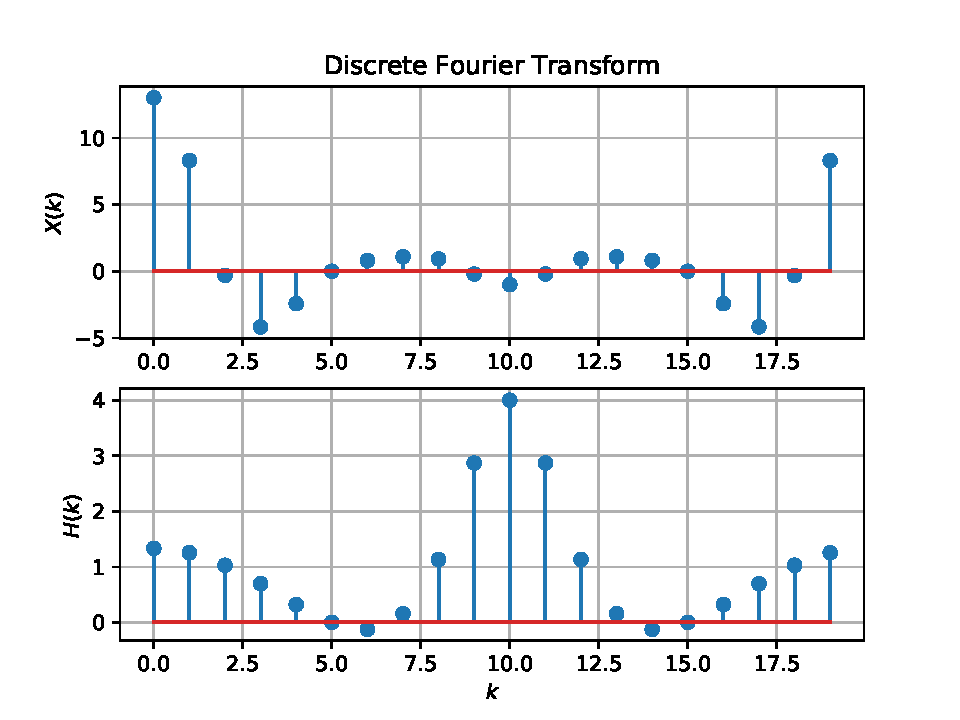
\includegraphics[width=\columnwidth]{/home/ubuntu/Desktop/Assign 1/6.1.pdf}
	\caption{Plots of the real parts of the DFT of $x(n)$ and $h(n)$}
	\label{fig:6.1}
\end{figure}
	
\item Compute 
\begin{equation}\label{6.2}
	Y(k) = X(k)H(k)
\end{equation}
\solution 
	%
\begin{lstlisting}
	wget https://github.com/omkar30122001/Assign_1/blob/main/6.2.py
\end{lstlisting}
\begin{figure}[!ht]
	\centering
	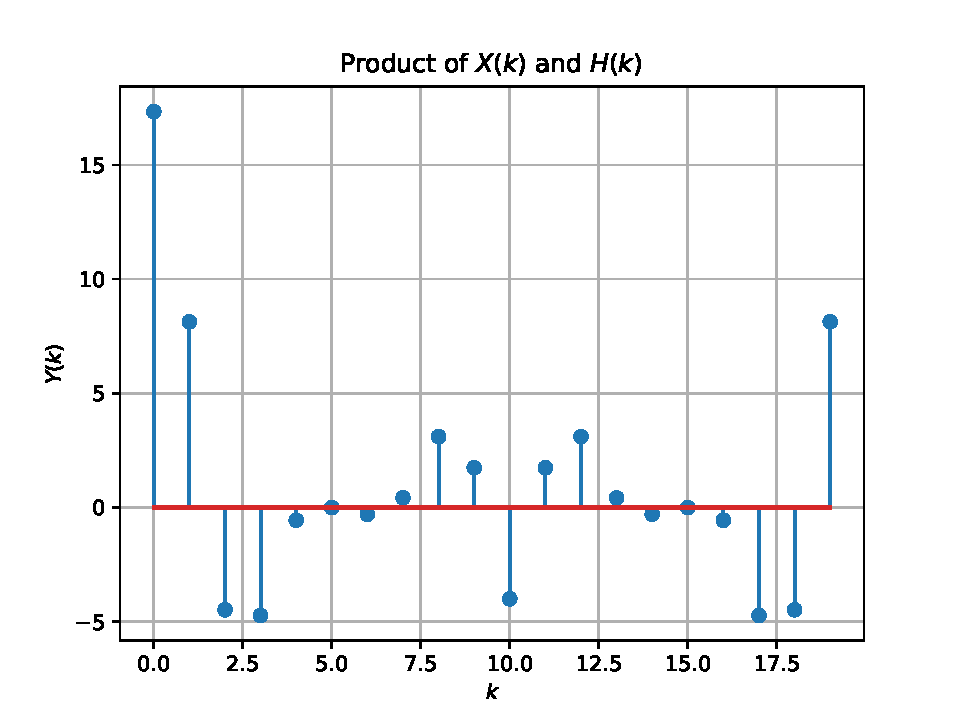
\includegraphics[width=\columnwidth]{/home/ubuntu/Desktop/Assign 1/6.2.pdf}
	\caption{$Y(k)$}
\end{figure}
\item Compute
\begin{equation} \label{6.3}
	y\brak{n}={\frac {1}{N}}\sum _{k=0}^{N-1}Y\brak{k}\cdot e^{\j 2\pi kn/N},\quad n = 0,1,\dots, N-1
\end{equation}
\\
\solution The following code plots Fig. \ref{fig:ynconv}. Note that this is the same as 
	$y(n)$ in  Fig.3.2 
%
\begin{lstlisting}
	wget https://github.com/omkar30122001/Assign_1/blob/main/6.3.py
\end{lstlisting}
	
\begin{figure}[!ht]
	\centering
	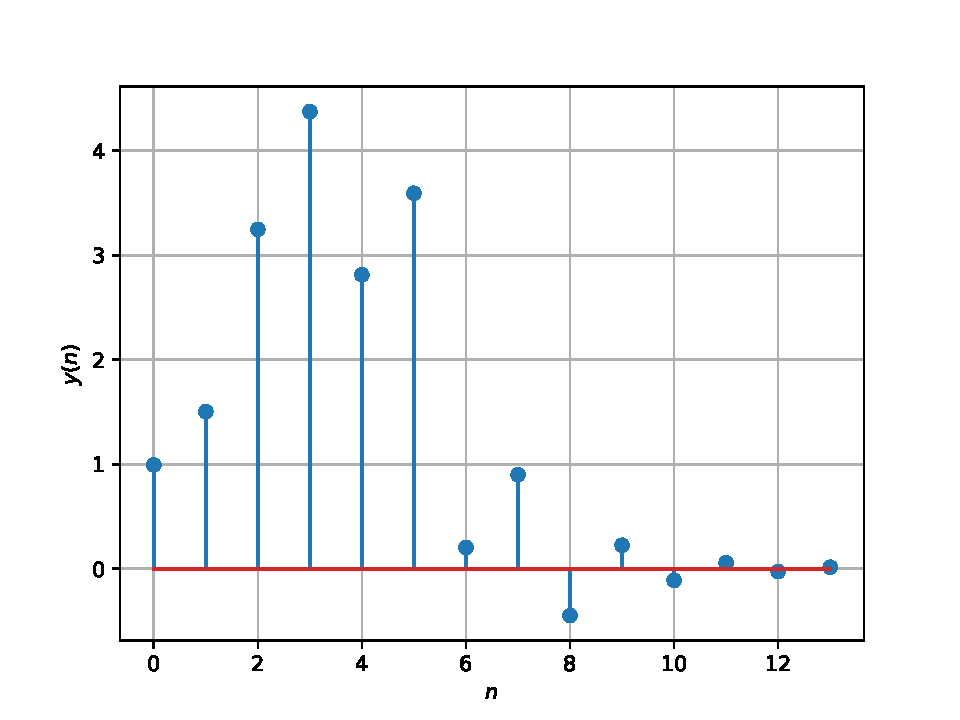
\includegraphics[width=\columnwidth]{/home/ubuntu/Desktop/Assign 1/6.3.pdf}
	\caption{$y(n)$ from the DFT}
	\label{fig:yndft}
\end{figure}
	
\item Repeat the previous exercise by computing $X(k), H(k)$ and $y(n)$ through FFT and 
IFFT.
\solution code:
\begin{lstlisting}
	wget https://github.com/omkar30122001/Assign_1/blob/main/6.4.py
\end{lstlisting}
Observe that Fig. \eqref{fig:y-n-fft} is the same as $y(n)$ in Fig.3.2
\begin{figure}
	\centering
	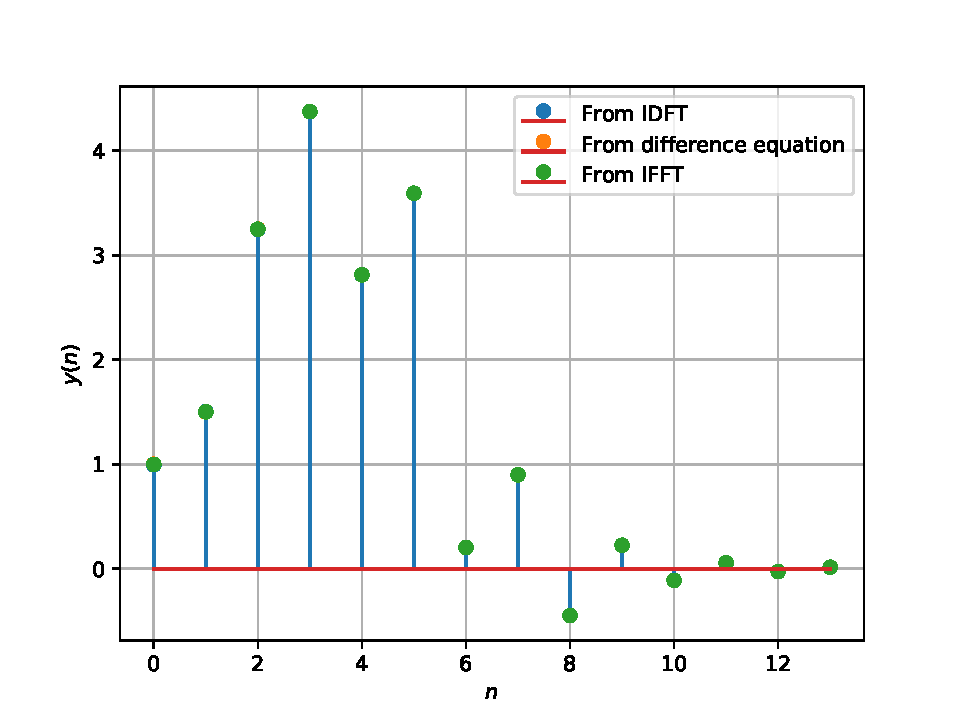
\includegraphics[width=\columnwidth]{/home/ubuntu/Desktop/Assign 1/6.4.pdf}
	\caption{$y(n)$ using FFT and IFFT}
	\label{fig:y-n-fft}
\end{figure}
%
\section{FFT}
% \subsection{Definitions}
\begin{enumerate}[label=\arabic*.,ref=\thesection.\theenumi]
	\numberwithin{equation}{section}
\item The DFT of $x(n)$ is given by
\begin{align}
	X(k) \triangleq \sum_{n=0}^{N-1} x(n) e^{-j 2 \pi k n / N}, \quad k=0,1, \ldots, N-1
\end{align}
\item Let 
\begin{align}
	W_{N} = e^{-j2\pi/N} 
\end{align}
Then the $N$-point {\em DFT matrix} is defined as 
\begin{align}
	\vec{F}_{N} = \sbrak{W_{N}^{mn}}, \quad 0 \le m,n \le N-1 
\end{align}
where $W_{N}^{mn}$ are the elements of $\vec{F}_{N}$.
\item Let 
\begin{align}
	\vec{I}_4 = \myvec{\vec{e}_4^{1} &\vec{e}_4^{2} &\vec{e}_4^{3} &\vec{e}_4^{4} }
\end{align}
be the $4\times 4$ identity matrix.  Then the 4 point {\em DFT permutation matrix} is defined as 
\begin{align}
	\vec{P}_4 = \myvec{\vec{e}_4^{1} &\vec{e}_4^{3} &\vec{e}_4^{2} &\vec{e}_4^{4} }
\end{align}
\item The 4 point {\em DFT diagonal matrix} is defined as 
\begin{align}
	\vec{D}_4 = diag\myvec{W_{8}^{0} & W_{8}^{1} & W_{8}^{2} & W_{8}^{3}}
\end{align}
\item Show that 
\begin{equation}
	W_{N}^{2}=W_{N/2}
\end{equation}
\solution
\begin{equation}
	W_{N} = e^{-\j2\pi/N}
\end{equation}
\begin{equation}
	\implies W_{N/2} = e^{-\j4\pi/N}
\end{equation}
And
\begin{equation}
	W_{N}^{2} = e^{-\j4\pi/N}
\end{equation}
\begin{equation}
	\boxed{W_{N}^{2} = W_{N/2}}
\end{equation}
%    \item Find $\vec{P}_6$.
%    \item Find $\vec{D}_3$.
\item Show that 
\begin{equation}
	\vec{F}_{4}=
	\begin{bmatrix}
		\vec{I}_{2} & \vec{D}_{2} \\
		\vec{I}_{2} & -\vec{D}_{2}
	\end{bmatrix}
	\begin{bmatrix}
		\vec{F}_{2} & 0 \\
		0 & \vec{F}_{2}
	\end{bmatrix}
	\vec{P}_{4}
\end{equation}
\solution
\begin{equation}
	\vec{F}_{2} = 
	\begin{bmatrix}
		W_{2}^0	&	W_{2}^0\\
		W_{2}^0	&	W_{2}^1
	\end{bmatrix}
	=		\begin{bmatrix}
		1	&	1\\
		1	&	-1
	\end{bmatrix}\\
\end{equation}
\begin{equation}
	\vec{D}_{4/2} =
	\begin{bmatrix}
		W_4^0 &	0\\
		0	&	W_4^1 
	\end{bmatrix}
	=\begin{bmatrix}
		1	&	0\\
		0	&	-i 
	\end{bmatrix}\\
\end{equation}
\begin{equation}
	\text{R.H.S } = 
	\begin{bmatrix}
		\vec{F}_{2} & \vec{D}_{4/2} \vec{F}_{2}\\
		\vec{F}_{2} & -\vec{D}_{4/2} \vec{F}_{2}\\
	\end{bmatrix}\vec{P}_{4}\\
\end{equation}
\begin{equation}
	=\begin{bmatrix}
		1	&	1	&	1	&	1\\
		1	&	-1	&	-i	&	i\\
		1	&	1	&	-1	&	-1\\
		1	&	-1	&	i	&	-i\\
	\end{bmatrix}\vec{P}_{4}\\
\end{equation}
\begin{equation}
	=\begin{bmatrix}
		1	&	1	&	1	&	1\\
		1	&	-i	&	-1	&	i\\
		1	&	-1	&	1	&	-1\\
		1	&	i	&	-1	&	-i\\
	\end{bmatrix}\\
\end{equation}
\begin{equation}
	\text{LHS} = \vec{F}_{4}
	= \begin{bmatrix}
		W_{4}^0	&	W_{4}^0	&	W_{4}^0	&	W_{4}^0\\
		W_{4}^0	&	W_{4}^1	&	W_{4}^2	&	W_{4}^3\\
		W_{4}^0	&	W_{4}^2	&	W_{4}^4	&	W_{4}^6\\
		W_{4}^0	&	W_{4}^3	&	W_{4}^6	&	W_{4}^9\\
	\end{bmatrix}\\
\end{equation}
\begin{equation}
	= \begin{bmatrix}
		1	&	1	&	1	&	1\\
		1	&	-i	&	-1	&	i\\
		1	&	-1	&	1	&	-1\\
		1	&	i	&	-1	&	-i\\
	\end{bmatrix}\\
\end{equation}
\text{Hence, LHS = RHS}
\item Show that 
\begin{equation}
	\vec{F}_{N}=
	\begin{bmatrix}
		\vec{I}_{N/2} & \vec{D}_{N/2} \\
		\vec{I}_{N/2} & -\vec{D}_{N/2}
	\end{bmatrix}
	\begin{bmatrix}
		\vec{F}_{N/2} & 0 \\
		0 & \vec{F}_{N/2}
	\end{bmatrix}
	\vec{P}_{N}
\end{equation}
\solution Observe that for even $N$ and letting $\vec{f}_N^i$ denote the $i^{\text{th}}$ column of $\vec{F}_N$, from 7.12 and 7.13,
\begin{align}
	\myvec{\vec{D}_{N/2}\vec{F}_{N/2} \\ -\vec{D}_{N/2}\vec{F}_{N/2}} = \myvec{\vec{f}_N^{2} & \vec{f}_N^{4} & \ldots & \vec{f}_N^{N}}
\end{align}
and
\begin{align}
	\myvec{\vec{I}_{N/2}\vec{F}_{N/2} \\ \vec{I}_{N/2}\vec{F}_{N/2}} = \myvec{\vec{f}_N^{1} & \vec{f}_N^{3} & \ldots & \vec{f}_N^{N - 1}}
\end{align}
Thus,
\begin{align}
	&\myvec{\vec{I}_2\vec{F}_2 & \vec{D}_2\vec{F}_2 \\ \vec{I}_2\vec{F}_2 & -\vec{D}_2\vec{F}_2} = \myvec{\vec{I}_{N/2} & \vec{D}_{N/2} \\ \vec{I}_{N/2} & -\vec{D}_{N/2}}\myvec{\vec{F}_{N/2} & 0 \\ 0 & \vec{F}_{N/2}} \nonumber \\
	&= \myvec{\vec{f}_N^{1} & \ldots & \vec{f}_N^{N - 1} & \vec{f}_N^{2} & \ldots & \vec{f}_N^{N}}
\end{align}
and so,
\begin{align}
	&\myvec{\vec{I}_{N/2} & \vec{D}_{N/2} \\ \vec{I}_{N/2} & -\vec{D}_{N/2}}\myvec{\vec{F}_{N/2} & 0 \\ 0 & \vec{F}_{N/2}}\vec{P}_{N} \nonumber \\
	&= \myvec{\vec{f}_N^{1} & \vec{f}_N^{2} & \ldots & \vec{f}_N^{N}} = \vec{F}_N
\end{align}
	\item Find 
	\begin{align}
		\vec{P}_4 \vec{x}
	\end{align}
	\solution
	\begin{equation}
		\vec{P_4} = \myvec{\vec{e_4}^{1} & \vec{e_4}^{3} & \vec{e_4}^{2} & \vec{e_4}^{4}}
	\end{equation}
	From \eqref{def:xn}
	\begin{equation}
		\vec{x} = \cbrak{1,2,3,4}
	\end{equation}
	\begin{equation}
		\vec{P}_{4}\vec{x} = \brak{1,3,2,4}
	\end{equation}
	\item Show that 
	\begin{align}
		\vec{X} = \vec{F}_N \vec{x}
		\label{eq:dft-mat-def}
	\end{align}
	where $\vec{x}, \vec{X}$ are the vector representations of $x(n), X(k)$ respectively.\\
	\solution
	\begin{align}
		\brak{\vec{F}_{N}\vec{x}}_{k} = \sum_{m=0}^{N-1}W_{N}^{mk}x(m)\\
		= \sum_{m=0}^{N-1} x(m) e^{-j 2 \pi k m / N}
		= X(k) = \vec{X}_{k} 
	\end{align}
	\item Derive the following Step-by-step visualisation  of
	8-point FFTs into 4-point FFTs and so on
	\begin{equation}
		\begin{bmatrix}
			X(0) \\ 
			X(1) \\ 
			X(2) \\ 
			X(3)
		\end{bmatrix}
		=
		\begin{bmatrix}
			X_{1}(0) \\ 
			X_{1}(1)\\ 
			X_{1}(2)\\
			X_{1}(3)\\
		\end{bmatrix}
		+
		\begin{bmatrix}
			W^{0}_{8} & 0 & 0 & 0\\
			0 & W^{1}_{8} & 0 & 0\\
			0 & 0 & W^{2}_{8} & 0\\
			0 & 0 & 0 & W^{3}_{8}
		\end{bmatrix}
		\begin{bmatrix}
			X_{2}(0) \\ 
			X_{2}(1) \\ 
			X_{2}(2) \\
			X_{2}(3)
		\end{bmatrix}
	\end{equation}
	\begin{equation}
		\begin{bmatrix}
			X(4) \\ 
			X(5) \\ 
			X(6) \\ 
			X(7)
		\end{bmatrix}
		=
		\begin{bmatrix}
			X_{1}(0) \\ 
			X_{1}(1)\\ 
			X_{1}(2)\\
			X_{1}(3)\\
		\end{bmatrix}
		-
		\begin{bmatrix}
			W^{0}_{8} & 0 & 0 & 0\\
			0 & W^{1}_{8} & 0 & 0\\
			0 & 0 & W^{2}_{8} & 0\\
			0 & 0 & 0 & W^{3}_{8}
		\end{bmatrix}
		\begin{bmatrix}
			X_{2}(0) \\ 
			X_{2}(1) \\ 
			X_{2}(2) \\
			X_{2}(3)
		\end{bmatrix}
	\end{equation}
	4-point FFTs into 2-point FFTs
	\begin{equation}
		\begin{bmatrix}
			X_{1}(0) \\ 
			X_{1}(1)\\ 
		\end{bmatrix}
		=
		\begin{bmatrix}
			X_{3}(0) \\ 
			X_{3}(1)\\ 
		\end{bmatrix}
		+
		\begin{bmatrix}
			W^{0}_{4} & 0\\
			0 & W^{1}_{4}
		\end{bmatrix}
		\begin{bmatrix}
			X_{4}(0) \\ 
			X_{4}(1) \\ 
		\end{bmatrix}
	\end{equation}
	\begin{equation}
		\begin{bmatrix}
			X_{1}(2) \\ 
			X_{1}(3)\\ 
		\end{bmatrix}
		=
		\begin{bmatrix}
			X_{3}(0) \\ 
			X_{3}(1)\\ 
		\end{bmatrix}
		-
		\begin{bmatrix}
			W^{0}_{4} & 0\\
			0 & W^{1}_{4}
		\end{bmatrix}
		\begin{bmatrix}
			X_{4}(0) \\ 
			X_{4}(1) \\ 
		\end{bmatrix}
	\end{equation}
	\begin{equation}
		\begin{bmatrix}
			X_{2}(0) \\ 
			X_{2}(1)\\ 
		\end{bmatrix}
		=
		\begin{bmatrix}
			X_{5}(0) \\ 
			X_{5}(1)\\ 
		\end{bmatrix}
		+
		\begin{bmatrix}
			W^{0}_{4} & 0\\
			0 & W^{1}_{4}
		\end{bmatrix}
		\begin{bmatrix}
			X_{6}(0) \\ 
			X_{6}(1) \\ 
		\end{bmatrix}
	\end{equation}
	\begin{equation}
		\begin{bmatrix}
			X_{2}(2) \\ 
			X_{2}(3)\\ 
		\end{bmatrix}
		=
		\begin{bmatrix}
			X_{5}(0) \\ 
			X_{5}(1)\\ 
		\end{bmatrix}
		-
		\begin{bmatrix}
			W^{0}_{4} & 0\\
			0 & W^{1}_{4}
		\end{bmatrix}
		\begin{bmatrix}
			X_{6}(0) \\ 
			X_{6}(1) \\ 
		\end{bmatrix}
	\end{equation}
	\begin{equation}
		P_{8}
		\begin{bmatrix}
			x(0) \\ 
			x(1) \\ 
			x(2) \\ 
			x(3) \\ 
			x(4) \\ 
			x(5) \\
			x(6) \\
			x(7)
		\end{bmatrix}
		= 
		\begin{bmatrix}
			x(0) \\ 
			x(2) \\ 
			x(4) \\ 
			x(6) \\
			x(1) \\ 
			x(3) \\ 
			x(5) \\
			x(7)
		\end{bmatrix}
	\end{equation}
	\begin{equation}
		P_{4}
		\begin{bmatrix}
			x(0) \\ 
			x(2) \\ 
			x(4) \\ 
			x(6) \\
		\end{bmatrix}
		= 
		\begin{bmatrix}
			x(0) \\ 
			x(4) \\ 
			x(2) \\
			x(6)
		\end{bmatrix}
	\end{equation}
	\begin{equation}
		P_{4}
		\begin{bmatrix}
			x(1) \\ 
			x(3) \\ 
			x(5) \\
			x(7)
		\end{bmatrix}
		= 
		\begin{bmatrix}
			x(1) \\ 
			x(5) \\ 
			x(3) \\ 
			x(7) \\
		\end{bmatrix}
	\end{equation}
	Therefore,
	\begin{equation}
		\begin{bmatrix}
			X_{3}(0) \\ 
			X_{3}(1)\\ 
		\end{bmatrix}
		= F_{2}
		\begin{bmatrix}
			x(0) \\ 
			x(4) \\ 
		\end{bmatrix}
	\end{equation}
	\begin{equation}
		\begin{bmatrix}
			X_{4}(0) \\ 
			X_{4}(1)\\ 
		\end{bmatrix}
		= F_{2}
		\begin{bmatrix}
			x(2) \\ 
			x(6) \\ 
		\end{bmatrix}
	\end{equation}
	\begin{equation}
		\begin{bmatrix}
			X_{5}(0) \\ 
			X_{5}(1)\\ 
		\end{bmatrix}
		= F_{2}
		\begin{bmatrix}
			x(1) \\ 
			x(5) \\ 
		\end{bmatrix}
	\end{equation}
	\begin{equation}
		\begin{bmatrix}
			X_{6}(0) \\ 
			X_{6}(1)\\ 
		\end{bmatrix}
		= F_{2}
		\begin{bmatrix}
			x(3) \\ 
			x(7) \\ 
		\end{bmatrix}
	\end{equation}
\solution We write out the values of performing an 8-point FFT on $\vec{x}$ as follows.
\begin{align}
	X(k) &= \sum_{n = 0}^{7}x(n)e^{-\frac{\j2kn\pi}{8}} \\
	&= \sum_{n = 0}^{3}\brak{x(2n)e^{-\frac{\j2kn\pi}{4}} + e^{-\frac{\j2k\pi}{8}}x(2n + 1)e^{-\frac{\j2kn\pi}{4}}} \\
	&= X_1(k) + e^{-\frac{\j2k\pi}{4}}X_2(k) 
\end{align}
where $\vec{X}_1$ is the 4-point FFT of the even-numbered terms and $\vec{X}_2$ is the 4-point FFT of the odd numbered terms. Noticing that for $k \geq 4$,
\begin{align}
	X_1(k) &= X_1(k - 4) \\
	e^{-\frac{\j2k\pi}{8}} &= -e^{-\frac{\j2(k - 4)\pi}{8}}
\end{align}
we can now write out $X(k)$ in matrix form as in 7.32 and 7.33. We also need to solve the two 4-point FFT terms so formed.
\begin{equation}
	X_1(k) = \sum_{n = 0}^{3}x_1(n)e^{-\frac{\j2kn\pi}{8}}
\end{equation}
\begin{equation}
	= \sum_{n = 0}^{1}\brak{x_1(2n)e^{-\frac{\j2kn\pi}{4}} + e^{-\frac{\j2k\pi}{8}}x_2(2n + 1)e^{-\frac{\j2kn\pi}{4}}}
\end{equation}
\begin{equation}	
	= X_3(k) + e^{-\frac{\j2k\pi}{4}}X_4(k) 
\end{equation}
using $x_1(n) = x(2n)$ and $x_2(n) = x(2n + 1)$. Thus we can write the 2-point FFTs
\begin{align}
	\begin{bmatrix}
		X_{3}(0) \\ 
		X_{3}(1)\\ 
	\end{bmatrix}
	= F_{2}
	\begin{bmatrix}
		x(0) \\ 
		x(4) \\ 
	\end{bmatrix} \\
	\begin{bmatrix}
		X_{4}(0) \\ 
		X_{4}(1)\\ 
	\end{bmatrix}
	= F_{2}
	\begin{bmatrix}
		x(2) \\ 
		x(6) \\ 
	\end{bmatrix}
\end{align}
Using a similar idea for the terms $X_2$, 
\begin{align}
	\begin{bmatrix}
		X_{5}(0) \\ 
		X_{5}(1)\\ 
	\end{bmatrix}
	= F_{2}
	\begin{bmatrix}
		x(1) \\ 
		x(5) \\ 
	\end{bmatrix} \\
	\begin{bmatrix}
		X_{6}(0) \\ 
		X_{6}(1)\\ 
	\end{bmatrix}
	= F_{2}
	\begin{bmatrix}
		x(3) \\ 
		x(7) \\ 
	\end{bmatrix}
\end{align}
But observe that from 7.25,
\begin{align}
	\vec{P}_8\vec{x} &= \myvec{\vec{x}_1\\\vec{x}_2} \\
	\vec{P}_4\vec{x}_1 &= \myvec{\vec{x}_3\\\vec{x}_4} \\ 
	\vec{P}_4\vec{x}_2 &= \myvec{\vec{x}_5\\\vec{x}_6}
\end{align}
where we define $x_3(k) = x(4k)$, $x_4(k) = x(4k + 2)$, $x_5(k) = x(4k + 1)$, and $x_6(k) = x(4k + 3)$ for $k = 0, 1$.
	\item For 
	\begin{align}
		\vec{x} = \myvec{1\\2\\3\\4\\2\\1}
		\label{eq:equation1}
	\end{align}
	compte the DFT  
	using 
	\eqref{eq:dft-mat-def} \\
	\solution
	\begin{align}
		\vec{X} = \vec{F}_6 \vec{x}
	\end{align}	
	\begin{align}
		= \begin{bsmallmatrix}
			1	&	1	&	1	&	1	&	1	&	1\\
			1	&	\brak{e^{\frac{-j2\pi}{6}}}	&	\brak{e^{\frac{-j2\pi}{6}}}^2	&	\brak{e^{\frac{-j2\pi}{6}}}^3	&	\brak{e^{\frac{-j2\pi}{6}}}^4	&	\brak{e^{\frac{-j2\pi}{6}}}^5\\
			1	&	\brak{e^{\frac{-j2\pi}{6}}}^2	&	\brak{e^{\frac{-j2\pi}{6}}}^4	&	\brak{e^{\frac{-j2\pi}{6}}}^6	&	\brak{e^{\frac{-j2\pi}{6}}}^8	&	\brak{e^{\frac{-j2\pi}{6}}}^{10}\\
			1	&	\brak{e^{\frac{-j2\pi}{6}}}^3	&	\brak{e^{\frac{-j2\pi}{6}}}^6	&	\brak{e^{\frac{-j2\pi}{6}}}^9	&	\brak{e^{\frac{-j2\pi}{6}}}^{12}	&	\brak{e^{\frac{-j2\pi}{6}}}^{15}\\
			1	&	\brak{e^{\frac{-j2\pi}{6}}}^4	&	\brak{e^{\frac{-j2\pi}{6}}}^8	&	\brak{e^{\frac{-j2\pi}{6}}}^{12}	&	\brak{e^{\frac{-j2\pi}{6}}}^{16}	&	\brak{e^{\frac{-j2\pi}{6}}}^{20}\\
			1	&	\brak{e^{\frac{-j2\pi}{6}}}^5	&	\brak{e^{\frac{-j2\pi}{6}}}^{10}	&	\brak{e^{\frac{-j2\pi}{6}}}^{15}	&	\brak{e^{\frac{-j2\pi}{6}}}^{20}	&	\brak{e^{\frac{-j2\pi}{6}}}^{25}
		\end{bsmallmatrix}
		\myvec{1\\2\\3\\4\\2\\1}
	\end{align}
	\begin{align}
		=\myvec{13\\-4 - \sqrt{3}j\\ 1\\-1\\1\\-4 + \sqrt{3}j}
	\end{align}
	\item Repeat the above exercise using the FFT
	after zero padding $\vec{x}$. \\
	\solution \\
	The code:
	\begin{lstlisting}
	wget https://github.com/omkar30122001/Assign_1/blob/main/7.12.py
	\end{lstlisting}
	The result:
	\begin{equation}
		\begin{bmatrix}
			13\\
			-3.1213-6.5355j\\
			j\\
			1.1213-0.5355j\\
			-1\\
			1.1213+0.5355j\\
			-j\\
			-3.1213+6.5355j
		\end{bmatrix}
	\end{equation}
	\item Write a C program to compute the 8-point FFT. \\
	\solution \\
	The code:
	\begin{lstlisting}
	wget https://github.com/omkar30122001/Assign_1/blob/main/7.13.c
	\end{lstlisting}
The output:
\begin{equation}
	\begin{bmatrix}
		13\\
		-3.1327 - j6.5545\\
		j\\
		1.1327 - j0.5545\\
		-1\\
		1.1327 + j0.5545\\
		- j\\
		-3.1327 + j6.5545\\
	\end{bmatrix}
\end{equation}
\end{enumerate}
\section{Exercises}
Answer the following questions by looking at the python code in Problem \ref{prob:output}.
\begin{enumerate}[label=\thesection.\arabic*]
	\item
	The command
	\begin{lstlisting}
	output_signal = signal.lfilter(b, a, input_signal)
	\end{lstlisting}
	in Problem \ref{prob:output} is executed through the following difference equation
	\begin{equation}
		\label{eq:iir_filter_gen}
		\sum _{m=0}^{M}a\brak{m}y\brak{n-m}=\sum _{k=0}^{N}b\brak{k}x\brak{n-k}
	\end{equation}
	%
	where the input signal is $x(n)$ and the output signal is $y(n)$ with initial values all 0. Replace
	\textbf{signal.filtfilt} with your own routine and verify.\\
	\solution \\
	\begin{lstlisting}
	wget https://github.com/omkar30122001/Assign_1/blob/main/8.1.py
	\end{lstlisting}
	%
	\item Repeat all the exercises in the previous sections for the above $a$ and $b$.
	\solution For the given values, the difference equation is
\begin{align*}
&y(n) - \brak{4.44}y(n - 1) + \brak{8.78}y(n - 2) \nonumber \\
&- \brak{9.93}y(n - 3) + \brak{6.90}y(n - 4) \nonumber \\
&- \brak{2.93}y(n - 5) \nonumber + \brak{0.70}y(n - 6) \nonumber \\
&- \brak{0.07}y(n - 7) = \brak{5.02 \times 10^{-5}}x(n) \nonumber \\
&+ \brak{3.52 \times 10^{-4}}x(n - 1)  \\
&+ \brak{1.05 \times 10^{-3}}x(n - 2) \nonumber \\
&+ \brak{1.76 \times 10^{-3}}x(n - 3) \\
&+ \brak{1.76 \times 10^{-3}}x(n - 4) \nonumber \\
&+ \brak{1.05 \times 10^{-3}}x(n - 5) \\
&+ \brak{3.52 \times 10^{-4}}x(n - 6) \nonumber \\
&+ \brak{5.02 \times 10^{-5}}x(n - 7)
\end{align*}
	From \eqref{eq:iir_filter_gen}, we see that the transfer function can be written as follows
	\begin{align}
		H(z) &= \frac{\sum_{k = 0}^{N}b(k)z^{-k}}{\sum_{k = 0}^{M}a(k)z^{-k}} \\
		&= \sum_{i}\frac{r(i)}{1 - p(i)z^{-1}} + \sum_{j}k(j)z^{-j}
		\label{eq:trans-func}
	\end{align}
	where $r(i)$, $p(i)$, are called residues and poles respectively of the partial 
	fraction expansion of $H(z)$. $k(i)$ are the coefficients of the direct polynomial 
	terms that might be left over. We can now take the inverse $z$-transform of (8.4) and get using \eqref{eq:anun},
	\begin{align}
		h(n) &= \sum_{i}r(i)[p(i)]^nu(n) + \sum_{j}k(j)\delta(n - j)
		\label{eq:h-n-expr}
	\end{align}
	Substituting the values,
	\begin{align}
		&h(n) = [\brak{2.76}\brak{0.55}^n \nonumber \\ 
		&+ \brak{-1.05-1.84\j}\brak{0.57+0.16\j}^n \nonumber \\
		&+ \brak{-1.05+1.84\j}\brak{0.57-0.16\j}^n \nonumber \\
		&+ \brak{-0.53+0.08\j}\brak{0.63+0.32\j}^n \nonumber \\
		&+ \brak{-0.53-0.08\j}\brak{0.63-0.32\j}^n \nonumber \\
		&+ \brak{0.20+0.004\j}\brak{0.75+0.47\j}^n \nonumber \\
		&+ \brak{0.20-0.004\j}\brak{0.75-0.47\j}^n]u(n) \nonumber \\
		&+ \brak{-6.81 \times 10^{-4}}\delta(n)
	\end{align}
	The values $r(i)$, $p(i)$, $k(i)$ and thus the impulse response function are computed and plotted at
	\begin{lstlisting}
	wget https://github.com/omkar30122001/Assign_1/blob/main/8.2.1.py
	\end{lstlisting}
	The filter frequency response is plotted at
	\begin{lstlisting}
	wget https://github.com/omkar30122001/Assign_1/blob/main/8.2.2.py
	\end{lstlisting}
	Observe that for a series $t_n = r^n$, $\frac{t_{n + 1}}{t_n} = r$.
	By the ratio test, $t_n$ converges if $|r| < 1$. We observe that for all $i$, 
	$|p(i)| < 1$ and so, as $h(n)$ is the sum of many convergent series,
	we see that $h(n)$ converges and is bounded.
	\begin{align}
		\sum_{n = 0}^{\infty}h(n) = H(1) = \frac{\sum_{k = 0}^{N}b(k)}{\sum_{k = 0}^{M}a(k)} = 1 < \infty
	\end{align}
	Therefore, the system is stable. From
	Fig. \eqref{fig:butter-imp}, $h(n)$ is negligible after $n \geq 64$, and we
	can apply a 64-bit FFT to get y(n). The following code uses the DFT matrix
	to generate $y(n)$ in Fig. \eqref{fig:butter-out}.
	\begin{lstlisting}
	wget https://github.com/omkar30122001/Assign_1/blob/main/8.2.3.py
	\end{lstlisting}
	\begin{figure}[!htb]
		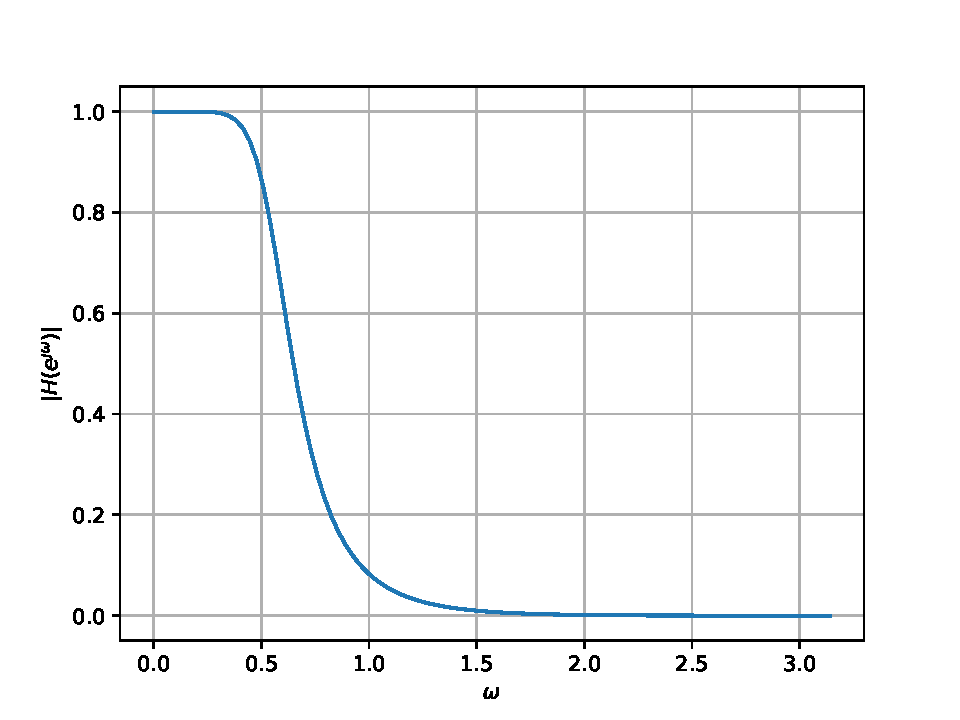
\includegraphics[width=\columnwidth]{/home/ubuntu/Desktop/Assign 1/8.2.1.pdf}
		\caption{Plot of $H(e^{\j\omega})$}
		\label{fig:butter-imp}
	\end{figure}
	\begin{figure}[!htb]
		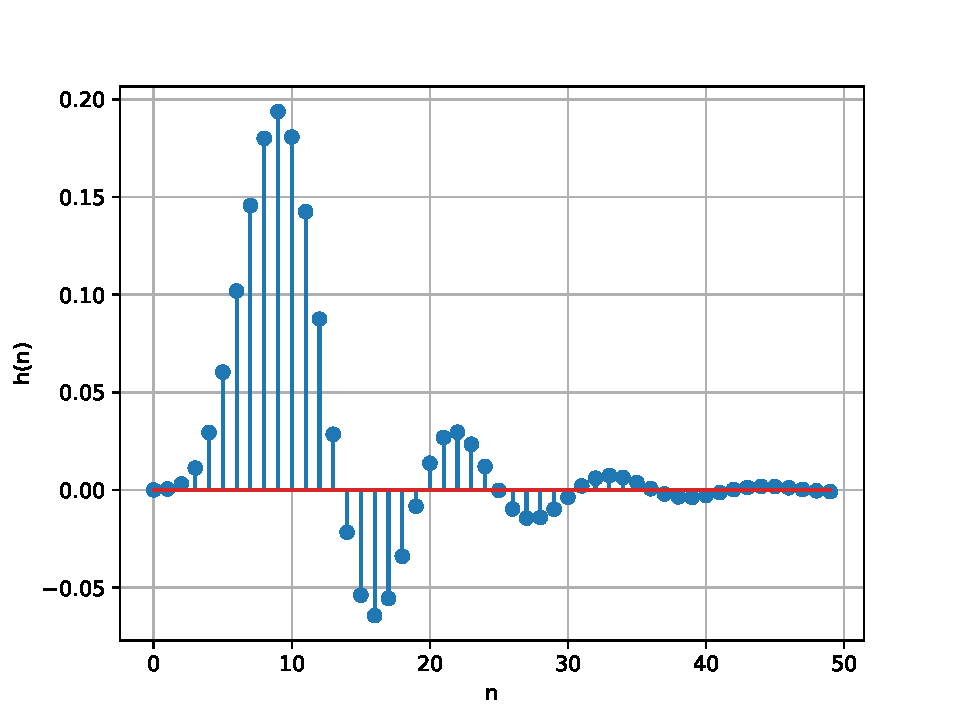
\includegraphics[width=\columnwidth]{/home/ubuntu/Desktop/Assign 1/8.2.2.pdf}
		\caption{Filter frequency response}
		\label{fig:butter-resp}
	\end{figure}
	\begin{figure}[!htb]
		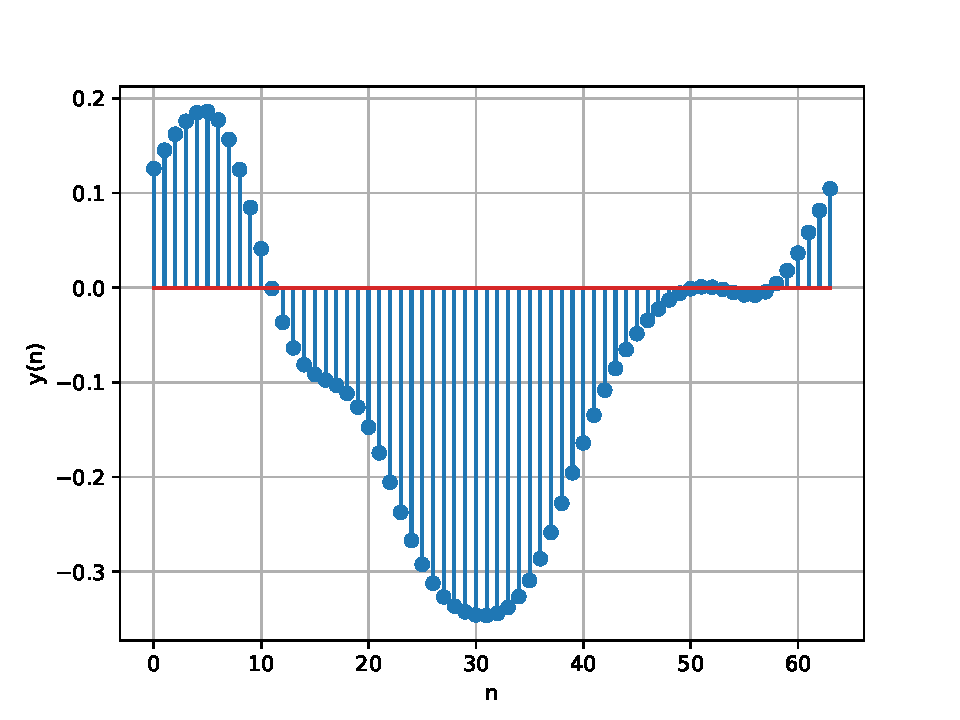
\includegraphics[width=\columnwidth]{/home/ubuntu/Desktop/Assign 1/8.2.3.pdf}
		\caption{Plot of $y(n)$}
		\label{fig:butter-out}
	\end{figure}
	
	\item What is the sampling frequency of the input signal?
	\\
	\solution
	Sampling frequency(fs)=44.1kHZ.
	\\ \\ \\ \\
	\item
	What is type, order and  cutoff-frequency of the above butterworth filter
	\\
	\solution
	The given butterworth filter is low pass with order=2 and cutoff-frequency=4kHz.
	%
	\item
	Modifying the code with different input parameters and to get the best possible output.
	 \\
	\solution
	We make the order of the filter = 7
	\\ The code:
	\begin{lstlisting}
	wget https://github.com/omkar30122001/Assign_1/blob/main/8.5.py
	\end{lstlisting}
\end{enumerate}
\end{enumerate}
\end{document}